\documentclass{article}

\usepackage{../../austin137}
\usepackage{../../local}
\usehyperstuff

\usepackage{wrapfig}

\begin{document}

%%%%%%%%%%%%%%%%%%%%%%%%%%%%%%%%%%%%%%%%%%%%%%%%%%%%%%%%%%%%%%%%%%%%%%%%%%%%%%%%
\addcopyright
\begin{center}
{\bf \large Physics W89 - Introduction to Mathematical Physics - Summer 2023}\\\medskip
{\bf \large Problem Set - Module 08 - An ODE to Differential Equations} \\\medskip
{\emph{Last Update: \today}}\\\medskip
{Student: Yutong Du}
\end{center}

\dphline
\bigskip
%%%%%%%%%%%%%%%%%%%%%%%%%%%%%%%%%%%%%%%%%%%%%%%%%%%%%%%%%%%%%%%%%%%%%%%%%%%%%%%%
\section*{Problem 8.1 - First-Order Linear Differential Equations}
\relevid{Linear ODEs and Linear Algebra;
First-Order Separable and Linear ODEs;
Systems of First-Order ODEs}


\paragraph{}
Consider a moving object subjected to a linear drag force, $F_{\textrm{drag}} = -\gamma v$.  This gives a linear first-order ordinary differential 
equation in the dependent variable $v$,
	\begin{equation}
		m\dot{v} = -\gamma v,	\qquad \gamma >0.
	\label{drag}
	\end{equation}
The negative sign means that when velocity is positive, the acceleration is negative and vice-versa, as would be expected.  
This could conceivably be used to describe, say, the motion of a billiard ball moving on a table after being struck.  Suppose our billiard ball of mass $m$
has initial velocity $v_{0}$.

%%%%%%%%%%%%%%%%%%%%%
\paragraph{(a)}
Solve the differential equation Eq.~\ref{drag} with the initial condition $v(0) = v_{0}$.
Sketch your solution.
Show that even though it takes an infinite amount of time for the billiard ball to fully stop, the ball only travels a finite distance.  
What is the total distance traveled by the ball?

\begin{solution}
	This differential equation is separable so we can separate and integrate:
	\begin{align*}
		m \dv{v}{t} &= -\gamma v\\
		\frac{\mathrm d v}{v} &= -\frac{\gamma}{m}\mathrm dt\\
		\therefore \ln v &=  -\frac{\gamma}{m}t + C \\
		v &=  e^{-\frac{\gamma}{m}t + C} 
	\end{align*}
	We can then write this as $e^{-\frac{\gamma}{m}t} e^C = Ae^{-\frac{\gamma}{m}t}$, and using our initial
	condition of $v(0) = v_0$, we get the full solution:
	\[
		v(t) = v_0e^{-\frac{\gamma}{m}t} 
	\] 
	We can see that since this is a decaying exponential, this will never reach zero, and so the ball will 
	never fully stop. But, the distance travelled can be calculated by taking the integral of this 
	from 0 to infinity:
	\[
	D = \int_0^\infty v_0e^{-\frac{\gamma}{m}t} = \left[-\frac{m}{\gamma}v_0e^{-\frac{\gamma}{m}t}\right]_0^\infty = 0 - \left( -\frac{m}{\gamma}v_0 \right)= \frac{m}{\gamma} v_0
	\] 
\end{solution}
\phline
%%%%%%%%%%%%%%%%%%%%%
\paragraph{}
The solution to a general inhomogeneous first-order linear differential equation $\dot{y} + p(t)y = q(t)$ with initial condition $y(0) = y_{0}$ is given by
	\begin{equation}
		y(t) = e^{-\mathcal{I}(t)}\int_{0}^{t}q(t')e^{+\mathcal{I}(t')}dt' + y_{0}e^{-\mathcal{I}(t)},	\qquad	\mathcal{I}(t) \equiv \int_{0}^{t} p(t')dt'.
	\label{linearsoln}
	\end{equation}

\paragraph{(b)}
Show explicitly that Eq.~\ref{linearsoln} solves the differential equation and gives the correct initial condition. 

\begin{solution}
	I'll do the initial condition first. If we plug in $t = 0$, the first term disappears, since 
	the integral is of zero width. For the second term, our $e^{-I(t)} = e^0 = 1$ (again, 
	$I(t)$ is defined as an integral, and when we plug in $t = 0$ it is again another integral
	of zero width.), so we only get $y_0$ out, as desired. 

	Now to verify the solution. First, we recall the relation:
	\[
		\dv{x} \int_0^x f(x') dx' = f(x)
	\] 
	This will prove useful later on in the problem when we invoke the chain rule, since we'll need the 
	following derivative: 
	\[
		I(t) = \int_0^t p(t') dt' \implies \dv{I}{t} = p(t)
	\] 
	Now, we have to take the derivative, which is a really big product rule and chain rule application:
	\begin{align*}
		\dot y &= \dv{t} \left[ e^{-I(t)} \int_0^t q(t') e^{I(t')} dt' + y_0e^{-I(t)}\right]\\
			   &= \dv{t}(e^{-I(t)}) \int_0^t q(t') e^{I(t')} dt' + e^{-I(t)} \dv{t}\int_0^t q(t') e^{I(t')} dt' + y_0 \dv{t} e^{-I(t)} \\
			   &= -e^{-I(t)} \dv{I}{t} \int_0^t q(t') e^{I(t')} dt' + e^{-I(t)} q(t) e^{I(t)} + y_0e^{-I(t)}\dv{I}{t} \\
			   &= -e^{-I(t)}p(t) \int_0^t q(t') e^{I(t')} dt' + q(t) + y_0e^{-I(t)} p(t) 
	\end{align*}
	Now we plug this into the differential equation, and we see that everything cancels except for 
	$q(t)$: 
	\[
		-e^{-I(t)} p(t) \int_0^t q(t') e^{I(t')} dt' + q(t) - y_0 e^{-I(t)} p(t) + p(t)\left[
		e^{-I(t)} \int_0^t q(t') e^{I(t')} dt' + y_0e^{-I(t)}\right] = q(t) 
	\] 
	Therefore, since this equals $q(t)$, it solves the differential equation.
\end{solution}

\phline
%%%%%%%%%%%%%%%%%%%%%
\paragraph{}
Consider the following inhomogeneous linear ODE
	\begin{equation*}
		\frac{dy}{dx} = -y\cos x + \sin 2x,
	\end{equation*}
where $x$ is our independent variable.

\paragraph{(c)}
Find the functions $p(x)$ and $q(x)$ that put this into our standard first-order linear ODE form.  Next find the function $\mathcal{I}(x)$ and a general solution to 
the homogeneous version of this ODE.  Finally, find a general solution to the original inhomogeneous equation.
\extrasubpart{Explicitly check that your answer solves the ODE.}

\begin{solution}
	Rearranging this differential equation we get:
	\[
		\dv{y}{x} + y \cos x = \sin 2x
	\] 
	This means that we can now extract $p(x) = \cos x$ and $q(x) = \sin 2x$. Then, from lecture, we know that our
	homogeneous solution is of the form:
	\[
		y_h(x) = y_0e^{-\int_0^x p(x) dx} = y_0e^{-\sin x}
	\] 
	Then, the particular solution is of the form $y_p(x) = z(x)e^{-I(x)} = z(x) e^{-\sin x}$ (again, pulled
	straight from the notes), with $z(x)$ being:
	\[
		z(x) = \int_0^x q(x') e^{I(x')} dx' = \int_0^x \sin(2x') e^{\sin x'} dx
	\] 
	Here we can use the relation that $\sin(2x) = 2 \sin x \cos x$ to get:
	\begin{align*}
		z(x) &= \int_0^x 2 \sin x' \cos x' e^{\sin x'} dx\\
			 &= \int_0^{\sin x} 2ue^u du \\
			 &= 2 \left[ u e^u\right]_0^{\sin x} - 2\int_0^{\sin x} e^u du \\
			 &= 2(\sin x e^{\sin x} - (e^{\sin x} -1)) 
	\end{align*}
	Therefore, our particular solution is:
	\begin{align*}
		y_p(x) &= 2(1 + \sin x e^{\sin x} - e^{\sin x} )e^{-\sin x} \\
			   &= 2(e^{- \sin x} + \sin x - 1) 
	\end{align*} 
	Combining this with our homogeneous solution to get the general solution:
	\[
		y(x) = y_0e^{-\sin x} + 2(e^{-\sin x} + \sin x - 1)
	\] 
\end{solution}

\phline
%%%%%%%%%%%%%%%%%%%%%
\paragraph{}
Consider the coupled system of two linear homogeneous differential equations
	\begin{align*}
		\dot{y}_{1} &= -2\alpha y_{1} + \sqrt{3}\alpha y_{2}\\
		\dot{y}_{2} &= +\sqrt{3}\alpha y_{1}.
	\end{align*}
If we make the two-component vector $\vec{y} \doteq \begin{smpmatrix}{0.8} y_{1}\\y_{2}\end{smpmatrix}$ then this can be put into the form of a matrix equation,
	\begin{equation*}
		\frac{d\vec{y}}{dt} = \mathsf{P}\vec{y},	\eqimplies		\begin{pmatrix} \dot{y}_{1} \\ \dot{y}_{2} \end{pmatrix} = \begin{pmatrix} -2\alpha & \sqrt{3}\alpha \\ 
		\sqrt{3}\alpha & 0 \end{pmatrix}\begin{pmatrix} y_{1}\\y_{2}\end{pmatrix}.
	\end{equation*}

\paragraph{(d)}
Find the eigenvectors $\vec{v}_{i}$ and eigenvalues $\lambda_{i}$ of $\mathsf{P}$.  Show that $\vec{y}_{i}(t) = e^{\lambda_{i}t}\vec{v}_{i}$ is a solution to this system of ODEs
for each eigenvalue/eigenvector pair.
Finally, find the linear combination of these two solutions that solves the original system of ODEs with the initial condition 
$y_{1}(0) = 1; y_{2}(0)=0$.\\
\note{Be careful with indices here.  You may want to label the eigenvectors by their eigenvalues instead of indices 1 and 2 to avoid confusion with the two dependent
variables $y_{1}$ and $y_{2}$.}
\extrasubpart{Which of the two eigenvector solutions dominate as $t\gg 1$?}

\begin{solution}
	The eigenvalues and eigenvectors of this matrix are:
	\begin{align*}
		\lambda_1 &= -3\alpha & \lambda_2 &= \alpha\\
		\vec v_1 &= \begin{pmatrix} -\sqrt{3} \\ 1 \end{pmatrix} & \vec v_2 &= \begin{pmatrix} \frac{1}{\sqrt{3} } \\ 1 \end{pmatrix} 
	\end{align*}
	Now it's time to check the solutions $\vec y_i(t) = e^{\lambda_i t} \vec v_i$, starting with the first 
	eigenvector-eigenvalue pair. Here, we have:
	\[
		\vec y_1(t) = e^{-3 \alpha t}\begin{pmatrix} -\sqrt{3} \\1 \end{pmatrix} 
	\] 
	which we can then split into:
	\begin{align*}
		y_1 &= -\sqrt{3} e^{-3 \alpha t} \\
		y_2 &= e^{-3 \alpha t} 
	\end{align*}
	Confirming the top equation:
	\[
		3\sqrt{3} \alpha e^{-3 \alpha t} = -2\alpha(-\sqrt{3} e^{-3 \alpha t}) + \sqrt{3} \alpha e^{-3 \alpha t} 
		= 2\sqrt{3} \alpha e^{-3 \alpha t} + \sqrt{3} \alpha e^{-3 \alpha t} = 3\sqrt{3} \alpha e^{-3 \alpha t} \
		\checkmark
	\] 
	And now the bottom equation:
	\[
		-3 \alpha e^{-3 \alpha t} = \sqrt{3} \alpha (-\sqrt{3} \alpha e^{-3 \alpha t}) =
		-3 \alpha e^{-3 \alpha t}
		\ \checkmark 
	\] 
	Now for the second solution, we have:
	\begin{align*}
		y_1 &= \frac{1}{\sqrt{3} }e^{\alpha t} \\
		y_2 &= \frac{\alpha}{\sqrt{3} }e^{\alpha t}
	\end{align*}
	With that, let's first confirm the top equation:
	\[
		\frac{\alpha}{\sqrt{3} }e^{\alpha t} = -\frac{2\alpha}{\sqrt{3} }e^{\alpha t} +
		\sqrt{3} \alpha e^{\alpha t} =\alpha  e^{\alpha t} \left(-\frac{2}{\sqrt{3} } +
		\sqrt{3}\right) = \frac{\alpha}{\sqrt{3} }e^{\alpha t}  \ \checkmark
	\] 
	And finally the bottom equation:
	\[
		\alpha e^{\alpha t} = \sqrt{3} \alpha \frac{1}{\sqrt{3} }e^{\alpha t} = \alpha e^{\alpha t} \ \checkmark
	\] 
\end{solution}
\bigskip
\dphline
\pagebreak
%%%%%%%%%%%%%%%%%%%%%%%%%%%%%%%%%%%%%%%%%%%%%%%%%%%%%%%%%%%%%%%%%%%%%%%%%%%%%%%%
\section*{Problem 8.2 - Damping and Driving a Harmonic Oscillator}
\relevid{Homogeneous Higher-Order Linear ODEs;
Second-Order Linear ODEs with Constant Coefficients;
Particular Solutions - Undetermined Coefficients;
Particular Solutions - Variation of Parameters}

\paragraph{}
Consider the damped simple harmonic oscillator we first met in Problem 1.4.  This system is governed by the second order linear differential equation
	\begin{equation*}
		m\ddot{y} + 2m\gamma\dot{y} + ky = 0	\eqimplies		\ddot{y} + 2\gamma\dot{y} + \omega_{0}^{2}y = 0,
	\end{equation*}
where $\omega_{0} \equiv \sqrt{k/m}$.  It may help throughout this problem to define $\widetilde\omega \equiv \sqrt{\omega_{0}^{2}-\gamma^{2}}$.

%%%%%%%%%%%%%%%%%%%%%
\paragraph{(a)}
Use the \emph{ansatz} $e^{\lambda t}$ to find two (complex) linearly independent solutions to this system in the \heavydef{underdamped} case, $\gamma< \omega_{0}$.
Form linear combinations of these solutions to come up with two \emph{real} linearly independent solutions.
Let $\omega_{0} = 10\gamma$ and sketch graphs of the two solutions when $t>0$, marking where $t=1/\gamma$ and $t=2\pi/\omega_{0}$ occur.\\
\note{Feel free to generate your graphs using a graphing program.  You may let $\gamma = 1$ for simplicity when you are graphing.
Be sure to attach printouts of the relevant graphs.}

\begin{solution}
	Using the ansatz, we have the following derivatives:
	\[
		\dot y = \lambda e^{\lambda t}, \ \ddot y = \lambda^2 e^{\lambda t} 
	\] 
	So our differential equation becomes:
	\begin{align*}
		\lambda^2 e^{\lambda t} + 2 \gamma \lambda e^{\lambda t} + \omega_0^2 e^{\lambda t} &=  0 \\
		\lambda^2 + 2 \gamma \lambda + \omega_0^2 &= 0
	\end{align*}
	Using the quadratic formula we get:
	\[
	\lambda_\pm = \frac{-2 \gamma \pm \sqrt{4 \gamma^2 - 4(1)(\omega_0^2)}}{2} = -\gamma \pm i 
	\sqrt{\omega_0^2 - \gamma^2} = - \gamma \pm i \widetilde \omega
	\] 
	To make linearly independent solutions, we can first take the sum of these two equations:
	\[
		y_1'(t) = e^{-\gamma t}\left(e^{i \widetilde \omega t} + e^{-i \widetilde \omega t}\right) = 2e^{- \gamma t} \cos(\widetilde \omega t)
	\] 
	Similarly, we can take the difference to get a linearly independent solution:
	\[
		y_2'(t) = e^{- \gamma t}\left( e^{i \widetilde \omega t} - e^{-i \widetilde \omega t} \right) = 
		2ie^{- \gamma t} \sin(\widetilde \omega t)
	\] 
	Stripping away the constant factors, we get our new (now linearly independent) pair of solutions:
	\[
		y_1(t) = e^{-\gamma t} \cos(\widetilde \omega t) \  \ y_2(t) = e^{-\gamma t}\sin(\widetilde \omega t)
	\] 
	So we now have two linearly independent solutions. Now for the plots: I will use $\gamma = 1$, meaning
	that $\omega_0 = 10$, and hence $\widetilde \omega = \sqrt{9} =3$. I also used an amplitude of 3 so 
	we can see the oscillation for a longer period of time:
	\begin{center}
		\begin{tikzpicture}[domain=0:6, samples=200]
			\draw(0, 0) -- (6, 0);
			\draw(0, -3) -- (0, 3);
			\draw[color=blue] plot (\x, {3*exp(-\x)*cos(3*\x r)}) node[above] {$y_1(t) = 3e^{-t} \cos(3t)$};
			\draw[color=red] plot (\x, {3*exp(-\x)*sin(3*\x r)}) node[below] {$y_2(t) = 3e^{-t} \sin(3t)$};
			\draw[dotted] (1, 0) -- (1, -3) node[below] {$t = \frac{1}{\gamma} = 1$};
			\draw[dotted] (0.628, 0) -- (0.628, -4) node[below] {$t = \frac{2\pi}{\omega_0} = \frac{\pi}{5}$};
		\end{tikzpicture}
	\end{center}
	I'm not entirely sure why we were asked to label the $t = 1 / \gamma$ and $t = 2\pi / \omega_0$, there 
	doesn't seem to be anything special about these points? 
\end{solution}
%%%%%%%%%%%%%%%%%%%%%
\paragraph{(b)}
Suppose $\gamma = \sqrt{2}\omega_{0}$ (so the oscillator is \heavydef{overdamped}).  Solve the initial condition problem where $y_{0} = A$ and $v_{0} = B\omega_{0}$.
Sketch graphs of the solutions for $t>0$ in the four cases $B = 2A$, $B=0$, $B=-2A$, and $B = -6A$.
\spoilers{First find the general solution, which is a linear combination of two linearly independent solutions.  Then use the two initial conditions to set up a
linear system of two equations in two unknowns and use our old linear algebra techniques to solve!}

\begin{solution}
	For an overdamped oscillator, the square root is a real quantity, so
	\[
		\lambda_{pm} = -\gamma \pm \sqrt{2\omega_0^2 - \omega_0^2} = -\gamma \pm \omega_0
	\] 
	This leads to the solutions:
	\[
		y_1(t) = e^{(-\gamma + \omega_0)t} \  y_2(t) = e^{-(\gamma + \omega_0)t}
	\] 
	Thus the general solution is a linear combination of these two:
	\[
		y(t) = c_1 e^{(-\gamma + \omega_0)t} + c_2 e^{-(\gamma+ \omega_0)t}
	\] 
	where $c_1$ and $c_2$ are currently undetermined. To find the values of $c_1$ and $c_2$, we use our 
	two initial conditions. First, we have $y_0 = A$, which gives us the equation:
	\[
	A = c_1 + c_2
	\] 
	which gives $c_1 = A - c_2$. Then, the condition of $v_0 = B \omega_0$ gives us:
	\[
		(-\gamma + \omega_0)c_1 - (\gamma + \omega_0)c_2 = B\omega_0
	\] 
	We could solve this system using Gaussian elimination and our techniques we learned in linear algebra, but 
	the equation is relatively simple enough that straight substitution isn't too bad. Doing so, we get
	the final results:
	\[
		c_2 = \frac{-\gamma A + \omega_0A - B \omega_0}{2 \omega_0}
	\] 
	Now we plug in $\gamma = \sqrt{2} \omega_0$\footnote{I know I could have done this earlier, but in my 
	original work I left it as $\gamma$ until the final step so that's what I'm going to do here.} to give
	us:
	\[
	c_2 = \frac{A (1 - \sqrt{2}) + B}{2}
	\] 
	substituting back for $c_1$, we finally have:
	\[
		c_1 =  \frac{A(1 - \sqrt{2}) + B}{2} \ \ \  c_2 = A - \frac{A(1- \sqrt{2}) + B}{2} 
	\] 
	As for the plots, I'll set $A = 1$, then set $B$ accordingly. Also, I'll set $\omega_0 = 1$, so $\gamma = 
	\sqrt{2}$. I've color coded them to match the values of $c_1$ and $c_2$:
	\begin{center}
		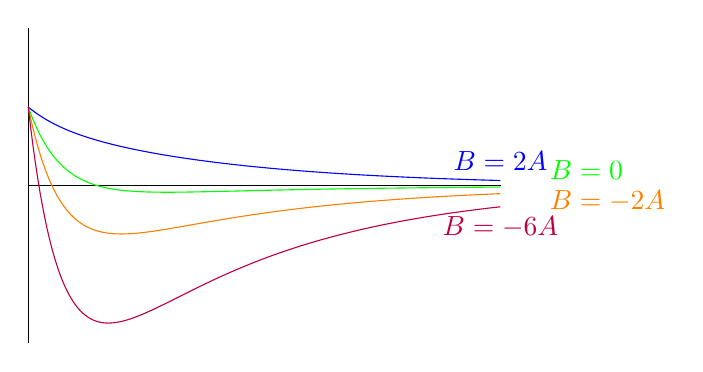
\begin{tikzpicture}[domain=0:6, samples=200]
			\draw(0, 0) -- (6, 0);
			\draw(0, -2) -- (0,2);
			\draw[color=blue] plot (\x,{0.792*exp(-0.414*\x)+0.207*exp(-2.414*\x)}) node[above] {$B = 2A$};
			\draw[color=green] plot (\x,{-0.207*exp(-0.414*\x)+1.207*exp(-2.414*\x)}) ;
			\draw[color=orange] plot (\x,{-1.207*exp(-0.414*\x)+2.207*exp(-2.414*\x)});
			\draw[color=purple] plot (\x,{-3.207*exp(-0.414*\x)+4.207*exp(-2.414*\x)})node[below] {$B = -6A$};
			\draw[color=green] (6.5, 0.2) node[right] {$B = 0$};
			\draw[color=orange] (6.5, -0.2) node[right] {$B = -2A$};
		\end{tikzpicture}
	\end{center}
\end{solution}

\phline
%%%%%%%%%%%%%%%%%%%%%
\paragraph{}
The \heavydef{critically damped} oscillator has $\gamma^{2} = \omega_{0}^{2}$.  Our ansatz $e^{\lambda t}$ in this case only returns a single solution 
$y_{h,1}(t) = e^{-\gamma t}$.  We can perform a reduction of order to find the second solution by using the ansatz $y_{h,2}(t) = c(t)y_{h,1}(t) 
= c(t)e^{-\gamma t}$.


\paragraph{(c)}
Plug this ansatz into the differential equation to come up with a differential equation for the function $c(t)$.  Solve this new equation to determine $y_{h,2}(t)$.  Verify that
$y_{h,2}(t)$ solves the differential equation.  Finally, sketch graphs of the two solutions for $t>0$.\\
\note{Remember that $\gamma=\omega_{0}$ in the critically damped case.}
\spoilers{You should find a second-order ODE for $c(t)$, but notice that $c(t)$ only occurs as a first or second derivative.  We can reduce the order of the ODE by
defining $d(t) = \dot{c}(t)$, in which case we have a first-order ODE for $d(t)$.}

\begin{solution}
	Computing the derivatives:
	\begin{align*}
		\dot y &= \dot c e^{- \gamma t} - c \gamma e^{- \gamma t}\\
		\ddot y &= \ddot c e^{- \gamma t} - \dot c \gamma e^{- \gamma t} - \dot c \gamma e^{-\gamma t} + 
		c \gamma^2 e^{- \gamma t} = \ddot c e^{- \gamma t} - 2 \dot c \gamma e^{- \gamma t} + c \gamma^2 
		e^{- \gamma t}
	\end{align*}
	So our differential equation becomes:
	\[
		\ddot c e^{- \gamma t} - 2 \dot c \gamma e^{- \gamma t} + c \gamma^2 e^{- \gamma t} + 
		2 \gamma\left( \dot c e^{- \gamma t} - c \gamma e^{- \gamma t}  \right) + \omega_0 c e^{- \gamma t} = 0
	\] 
	First we note that the $\dot c$ terms exactly cancel out. Further, using the fact that $\gamma^2 =
	\omega_0^2$, we find that the zeroth order $c$ terms also cancel exactly, giving us the differential 
	equation:
	\[
	\ddot c = 0 \implies c(t)= at + b
	\] 
	This is true because the most general kind of function whose second derivative is zero is a line. Further,
	we can actually get rid of the constants $a$ and $b$, since scaling by a constant factor and also adding
	two homogeneous solutions together always creates a homogeneous solution. This is to say, we don't need 
	the constants at all since we're after the \textit{simplest} solution. Thus, our second homogeneous 
	solution is of the form: 
	\[
		y_2(t) = te^{-\gamma t}
	\] 
	To verify this, we plug this back into the differential equation. First, taking the derivatives:
	\begin{align*}
		\dot y &= e^{-\gamma t} - \gamma te^{- \gamma t}  \\	
		\ddot y &= -2\gamma e^{-\gamma t} + \gamma^2 t e^{- \gamma t} 
	\end{align*}
	Thus:
	\[
	 -2\gamma e^{-\gamma t} + \gamma^2 t e^{- \gamma t} + 2\gamma\left[ e^{-\gamma t} - \gamma te^{- \gamma t}
	 \right] + \gamma^2 te^{- \gamma t} = -2\gamma e^{- \gamma t} + 2\gamma e^{- \gamma t} + 2\gamma^2 te^{- \gamma t} - 2 \gamma^2 t e^{- \gamma t} = 0
	\] 
	Since it equals zero after plugging in, we conclude that $y_2(t) = te^{-\gamma t}$ is a valid homogeneous
	solution. As for the plots of the two solutions, here they are (again, using $\gamma = 1$):
	\begin{center}
		\begin{tikzpicture}[domain=0:6, samples=200]
			\draw(0, 0) -- (6, 0);
			\draw(0, -2) -- (0,2);
			\draw[color=blue] plot (\x,{exp(-\x)}) node[above] {$y_1 = e^{-t}$};
			\draw[color=red] plot (\x,{\x*exp(-\x)}) node[below] {$y_2(t) = te^{-t}$};
		\end{tikzpicture}	
	\end{center}
\end{solution}


\phline
%%%%%%%%%%%%%%%%%%%%%
\paragraph{}
Now let's add a (complex) \heavydef{driving force} $F(t) = F_{0}e^{+i\omega t}$ to the oscillator! 
In this case the driving force acts as an inhomogeneity for the ODE governing the system, 
	\begin{equation}
		m\ddot{y} + 2m\gamma\dot{y} + m\omega_{0}^{2}y = F_{0}e^{+i\omega t}.
	\label{drivenunderdamped}
	\end{equation}
Suppose $\gamma<\omega_{0}$ so the oscillator is underdamped.

\paragraph{(d)}
Use the method of undetermined coefficients to find a particular (complex) solution to Eq.~\ref{drivenunderdamped}.  

\begin{solution}
	The method of undetermined coefficients says that when our inhomogeneity is an exponential, our guess should 
	be of the form $y = Ce^{i \omega t}$, where the coefficient in front of the exponential matches that of 
	the inhomogeneity. Computing derivatives:
	\begin{align*}
		\dot y &= i \omega Ce^{i \omega t}\\
		\ddot y &= - \omega^2 Ce^{i \omega t} 
	\end{align*}
	Plugging this into the differential equation, we get:
	\begin{align*}
		-m \omega^2 Ce^{i \omega t} + 2m \gamma i \omega C e^{i \omega t} + m \omega_0^2 C e^{i \omega t} &= 
		F_0 e^{i \omega t}\\
		C(-m \omega^2 + 2m \gamma i \omega + m \omega_0^2) &=  F_0
	\end{align*}
	This leads to the solution:
	\[
	C(\omega) = \frac{F_0}{m(\omega_0^2 - \omega^2 + 2 \gamma i \omega) }
	\] 
\end{solution}

%%%%%%%%%%%%%%%%%%%%%
\paragraph{(e)}
Your answer from part (d) should have been of the form $C(\omega)\,e^{i\omega t}$ where $C$ is a complex function of $\omega$.  
Find $\abs{C(\omega)}$, the magnitude of your particular solution as a function of the
driving frequency $\omega$.  Sketch a graph of the $\abs{C(\omega)}$ vs. $\omega$.  At what $\omega$ is the amplitude of the particular solution the greatest?

\begin{solution}
	Since $C(\omega)$ is a complex valued function, we have $|C(\omega)| = \sqrt{ C(\omega) C^*(\omega)}$. 
	I'll forget the square root now and derive $|C(\omega)|^2$, just to simplify my life a bit. Thus we have:
	\begin{align*}
		|C(\omega)|^2 &= \frac{F_0^2}{m^2}\left[\frac{1}{\omega_0^2 - \omega^2 + 2\gamma i \omega} \cdot 
		\frac{1}{\omega_0^2 - \omega^2 - 2 \gamma i \omega}\right]
	\end{align*}
	We can simplify the algebra a bit by letting $\omega' = \omega_0^2 - \omega^2$:
	\begin{align*}
		|C(\omega)|^2 &= \frac{F_0^2}{m^2}\left[(\omega' + 2 i \gamma \omega)(\omega' - 
		2 i \gamma \omega)\right]^{-1} \\
					&= \frac{F_0^2}{m^2}\left[ \omega'^2 + 4 \gamma^2 \omega^2 \right]^{-1}\\
					&= \frac{F_0^2}{m^2}\left[(\omega_0^2 - \omega^2)^2 + 4 \gamma^2 \omega^2\right]^{-1} 
	\end{align*}
	To make the expression a little bit more visually appealing:
	\[
		|C(\omega)| = \left[\frac{F_0^2}{m^2\left[(\omega_0^2 - \omega^2)^2 + 4 \gamma^2 \omega^2\right]}\right]^{1 / 2}
	\] 
	For the plot, just to make everything as simple as possible, we'll let all constants (except $\omega_0$, 
	which I'll vary) equal to 1, and I'll 
	also plot $|C(\omega)|^2$ since the equation is much nicer to type. I'll also set the 
	value of $\frac{F_0}{m} = 50$, so that the graph looks nicer. (I noticed that a smaller factor makes the 
	graph look too squished and it's hard to make out any detail) This won't change any 
	properties of the graph, since it's just a scaling factor. Therefore, we are plotting: 
	\[
	|C(\omega)|^2 = \frac{50}{(\omega_0^2-\omega^2)^2 + 4\omega^2}
	\] 
	The plot is below: 
	\begin{center}
		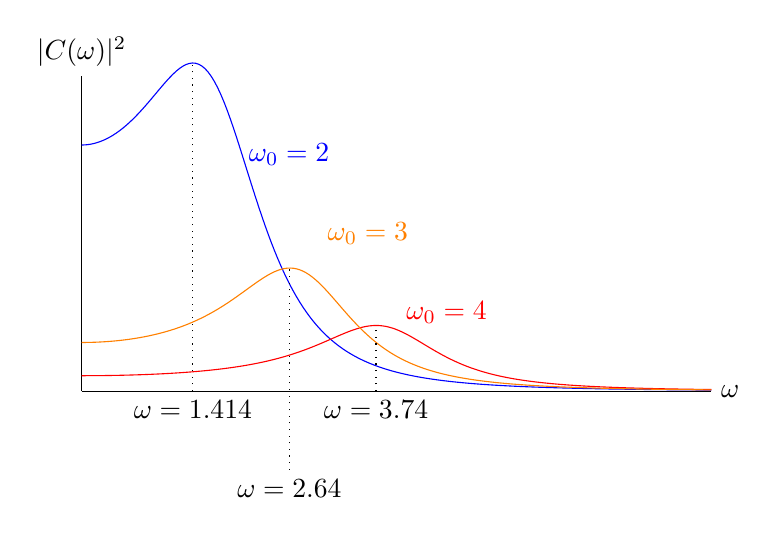
\begin{tikzpicture}[domain=0:8, samples=200]
			\draw(0, 0) -- (8, 0) node[right] {$\omega$}; 
			\draw(0, 0) -- (0,4) node[above] {$|C(\omega)|^2$};
			\draw[color=blue] plot (\x, {50/((4-\x^2)^2 + 4*\x^2)});
			\draw[color=red] plot (\x, {50/((16-\x^2)^2 + 4*\x^2)});
			\draw[color=orange] plot (\x, {50/((9-\x^2)^2 + 4*\x^2)});
			\draw[dotted] (2.64, -1) node[below] {$\omega = 2.64$} -- (2.64, 1.56);
			\draw[dotted] (1.414, 0) node[below] {$\omega = 1.414 $} -- (1.414, 4.16); 
			\draw[dotted] (3.74, 0) node[below] {$\omega = 3.74$}-- (3.74, 0.83);
			\draw[color=blue] (2, 3) node[right] {$\omega_0 = 2$};
			\draw[color=red] (4, 1) node[right] {$\omega_0 = 4$};	
			\draw[color=orange] (3, 2) node[right] {$\omega_0 = 3$};
		\end{tikzpicture}
	\end{center}
	Although this plot is rather crude, what I did want to show with this was that as our driving frequency 
	$\omega$ approaches 
	the frequency of the oscillator $\omega_0$, our amplitude reaches a maximum. This also makes physical 
	sense, since it's equivalent to propelling a swing -- we want to time our pushes with the frequency 
	of the swing in order to achieve maximum height.  

	As a bit of extra stuff, I also went ahead and threw $\omega_0 = 20$ into Mathematica, which generated
	the following plot:
	\begin{center}
		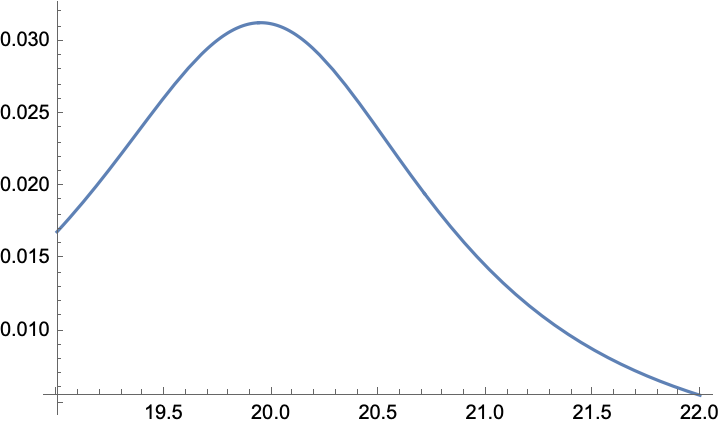
\includegraphics[scale=1]{2e.png}
	\end{center}
	this has a maximum at $\omega = 19.94$, which is more demonstration that this function is maximized at 
	$\omega \approx \omega_0$.
\end{solution}
\paragraph{}
\noindent\emph{Commentary: The homogeneous solutions from part (d) both exponentially decay and are therefore known as \heavydef{transient solutions}.  
After a few time constants, the particular solution is all that remains and is therefore known as the \heavydef{steady state solution}.  The frequency you found in (e) is called the
\heavydef{resonance frequency}.}

\phline
%%%%%%%%%%%%%%%%%%%%%
\paragraph{}
Finally, consider a \emph{critically damped} driven harmonic oscillator ($\omega_{0}=\gamma$) with an exponentially decaying driving force $F(t) = F_{0}e^{-\gamma t}$.
	\begin{equation}
		m\ddot{y} + 2m\gamma\dot{y} + m\gamma^{2}y = F_{0}e^{-\gamma t}.
	\end{equation}

\paragraph{(f)}
Use the method of {variation of parameters} to find a particular solution to the critically damped, driven harmonic oscillator.
\spoilers{The two homogeneous solutions you found in (c) should be $e^{-\gamma t}$ and $te^{-\gamma t}$.}

\begin{solution}
	First we divide both sides by $m$ so we can apply the variation of parameters:
	\[
		\ddot y + 2 \gamma \dot y + \gamma^2 \dot y = \frac{F_0}{m}e^{- \gamma t}
	\] 
	Our two homogeneous solutions are $e^{-\gamma t}$ and $te^{- \gamma t}$. Fortunately since this is a 
	second order differential equation, we have the result partially from lecture already. First, we 
	form the Wronskian (after some algebraic simplifications):
	\[
		W(t) = \begin{vmatrix} e^{- \gamma t} & te^{- \gamma t}\\ -\gamma e^{- \gamma t} & e^{- \gamma t} - \gamma te^{- \gamma t}\end{vmatrix} = e^{- 2 \gamma t} (1 - \gamma t) + \gamma t e^{- 2 \gamma t} = e^{- 2 \gamma t}
	\] 
	Now, we have our general solution:
	\[
		y(t) = c_1(t)y_{h 1}(t) + c_2(t) y_{h 2}(t)
	\] 
	where we have:
	\[
		\dot c_1(t) = \frac{\det \begin{pmatrix} 0 & te^{- \gamma t} \\ \frac{F_0}{m}e^{- \gamma t} & e^{- \gamma t} - \gamma t e^{- \gamma t} \end{pmatrix}}{W(t)} = \frac{1}{e^{-2 \gamma t}}\left(-\frac{F_0}{m}te^{- 2 \gamma t}\right) = -\frac{F_0}{m}t
	\]
	This means that:
	\[
	\dot c_1(t) = -\frac{F_0}{m}t \implies c_1(t) = -\frac{F_0}{2m}t^2
	\] 
	Now for $c_2(t)$:
	\begin{align*}
		\dot c_2(t) =  \frac{\det \begin{pmatrix} e^{- \gamma t} & 0\\ -\gamma e^{- \gamma t} & \frac{F_0}{m}e^{- \gamma t} \end{pmatrix}}{W(t)} = \frac{1}{e^{-2 \gamma t}}\left[e^{- \gamma t} \frac{F_0}{m}e^{- \gamma t}\right]
		= \frac{F_0}{m}
	\end{align*}
	And so we conclude: 
	\[
	\dot c_2(t) = \frac{F_0}{m}\implies c_2(t) = \frac{F_0}{m}t
	\] 
	Therefore, our particular solution is:
	\[
		y_p(t) = -\frac{F_0}{2m}t^2 e^{- \gamma t} + \frac{F_0}{m} t \cdot te^{- \gamma t} = \frac{F_0}{2m}t^2 e^{- \gamma t}
	\] 
\end{solution}

\bigskip
\dphline
\pagebreak
%%%%%%%%%%%%%%%%%%%%%%%%%%%%%%%%%%%%%%%%%%%%%%%%%%%%%%%%%%%%%%%%%%%%%%%%%%%%%%%%
\section*{Problem 8.3 - Linear Higher-Order ODEs}
\relevid{Homogeneous Higher-Order Linear ODEs;
Particular Solutions - Undetermined Coefficients;
Particular Solutions - Variation of Parameters;
Changing Variables}

%%%%%%%%%%%%%%%%%%%%%
\paragraph{(a)}
Use the Wronskian to show that $\{e^{\lambda_{1}t},e^{\lambda_{2}t},e^{\lambda_{3}t}\}$ is a set of three linearly independent functions if $\lambda_{1}$, $\lambda_{2}$,
and $\lambda_{3}$ are all distinct.

\begin{solution}
	This was done in a previous homework, so I'll just copy paste what I had from there. The Wronskian matrix is
:
	\[
		\mathbb W = \begin{pmatrix} e^{\lambda_1 x} & e^{\lambda_2x} & e^{\lambda_3x}\\
		\lambda_1 e^{\lambda_1x} & \lambda_2e^{\lambda_2x} & \lambda_3e^{\lambda_3x}\\
	\lambda_1^2 e^{\lambda_1x} & \lambda_2^2 e^{\lambda_2x} & \lambda_3^2e^{\lambda_3x}\end{pmatrix}
	\]
	So now we take the determinant
	\begin{multline*}
		\det(\mathbb W) = e^{\lambda_1x}\left( \lambda_2\lambda_3^2 e^{(\lambda_2 + \lambda_3)x} - \lambda_3\lambda_2^2
			e^{(\lambda_2 + \lambda_3)x}\right) +
			e^{\lambda_2x} \left( \lambda_1 \lambda_3^2 e^{(\lambda_1 + \lambda_3)x} - \lambda_3\lambda_1^2
		e^{(\lambda_1 + \lambda_3)x}\right) \\
		+ e^{\lambda_3 x}\left(\lambda_1\lambda_2^2 e^{(\lambda_1 + \lambda_2)x} -
			\lambda_2\lambda_1^2 e^{(\lambda_1 + \lambda_2)x}\right)
	\end{multline*}
	Simplifying:
	\begin{align*}
		\det(\mathbb W) &= e^{\lambda_1x}e^{(\lambda_2 +\lambda_3)x}\left( \lambda_2\lambda_3^2 -
		\lambda_3\lambda_2^2\right) + e^{\lambda_2x} e^{(\lambda_1 + \lambda_3)x} \left( \lambda_1\lambda_3^2 -
		\lambda_3\lambda_1^2\right) + e^{\lambda_3x}e^{(\lambda_1 + \lambda_2)x}\left( \lambda_1 \lambda_2^2 -
			\lambda_2 \lambda_1^2\right)\\
		&= e^{(\lambda_1 + \lambda_2 + \lambda_3)x} \left[ \lambda_2\lambda_3(\lambda_3 - \lambda_2) +
		\lambda_1 \lambda_3(\lambda_3 - \lambda_1) + \lambda_1 \lambda_2(\lambda_2 - \lambda_1)\right]
	\end{align*}
	If the three $\lambda$s are distinct, then at most one of them is zero, but this would always leave
	one of the terms unaffected, since each individual term only contains two of the three $\lambda$s.
	Specifically, the term that is unaffected will be the one that doesn't contain that particular $\lambda$
	that equals zero. This would still guarantee that the Wronskian is always nonzero, since this means
	there will be at least one nonzero term, and $e^{(\lambda_1 + \lambda_2 + \lambda_3)x}$ is never zero
	since it's an exponential function. So in the end, we will have an exponential (nonzero) multiplied with
	the square brackets (also nonzero), which will always result in a nonzero number.

	Since the Wronskian is never zero, we conclude that the functions are linearly independent.
\end{solution}

\paragraph{}
\noindent\emph{Commentary: An analogous can be proven for an arbitrary number of exponentials.  The Wronskian becomes what is known as a \heavydef{Vandermonde determinant} and 
evaluates to $\scalemath{0.8}{\prod_{1\leq i<j\leq n}} (\lambda_{j}-\lambda_{i})$ which is zero if any pair of $\lambda$s are the same and non-zero if all $\lambda$s are distinct..}

\phline
%%%%%%%%%%%%%%%%%%%%%
\paragraph{}
Consider the third-order homogeneous ODE
	\begin{equation}
		\dddot{y} - 2\ddot{y} - \dot{y} + 2y= 0.
	\label{thirdorder}
	\end{equation}

\paragraph{(b)}
Use the ansatz $y = e^{\lambda t}$ to find the general solution to Eq.~\ref{thirdorder}.  Your answer should be a linear
combination of three linearly independent functions.  Argue that the three functions you get are indeed linearly independent.

\begin{solution}
	First we calculate the derivatives:
	\begin{align*}
		\dot y &= \lambda e^{\lambda t}\\
		\ddot y &= \lambda^2 e^{\lambda t} \\
		\dddot y &= \lambda^3 e^{\lambda t}
	\end{align*}
	Plugging this in to the differential equation, we get:
	\begin{align*}
		\lambda^3 e^{\lambda t} - 2 \lambda^2 e^{\lambda t} - \lambda e^{\lambda t} + 2e^{\lambda t} &= 0\\
		\lambda^3 - 2\lambda^2 - \lambda + 2 &=  0 \\
		\lambda^2(\lambda - 2) - (\lambda - 2) &=  0 \\
		(\lambda - 2)(\lambda +1)(\lambda -1) &= 0
	\end{align*}
	So we get that $\lambda = 2, 1, -1$ are our solutions. This means that our three functions are $\{e^{2t}, 
	e^{t}, e^{-t}\}$. From the previous part, since each $\lambda$ is distinct, then we know that 
	these functions must be linearly independent.
\end{solution}
%%%%%%%%%%%%%%%%%%%%%
\paragraph{(c)}		\extrapart
Find the solution to the ODE from (b) under the initial conditions $y(0) = y_{0}$, $\dot{y}(0) = v_{0}$, $\ddot{y}_{0} = a_{0}$.

\phline
%%%%%%%%%%%%%%%%%%%%%
\paragraph{}
Consider the ODE from Eq.~\ref{thirdorder} with an inhomogeneity,
	\begin{equation}
		\dddot{y} - 2\ddot{y} - \dot{y} + 2y= 30e^{-t}.
	\label{thirdorderinhom}
	\end{equation}
	
\paragraph{(d)}
Find a particular solution to Eq.~\ref{thirdorderinhom}.
\spoilers{The inhomogeneity is already one of the homogeneous solutions, so if you are using the method of undetermined coefficients, you should try multiplying your ansatz by a factor
of $t$.  That is, use the trial solution $Cte^{-t}$ instead of just $Ce^{-t}$.}

\begin{solution}
	We use the spoiler here, and use the trial of $Cte^{-t}$. Computing derivatives:
	\begin{align*}
		\dot y &= Ce^{-t} - Cte^{-t}\\
		\ddot y &= -2Ce^{-t} + Cte^{-t} \\
		\dddot y &= 3Ce^{-t} - Cte^{-t}
	\end{align*}
	Plugging this in:
	\begin{align*}
		3Ce^{-t} - Cte^{-t} - 2\left( Cte^{-t} - 2Ce^{-t} \right) - \left( Ce^{-t} - Cte^{-t} \right) + 
		2Cte^{-t} &= 30 e^{-t}\\
		3Ce^{-t} + 4Ce^{-t} - Ce^{-t} &=  30e^{-t} \\
		6Ce^{-t} &= 30e^{-t} \\
		\therefore C = 5
	\end{align*}
	Therefore, we conclude that $y = 5te^{-t}$ is a particular solution.
\end{solution}

\phline
%%%%%%%%%%%%%%%%%%%%%
\paragraph{(e)}		\extrapart
Use the ansatz $y = e^{\lambda t}$ to find the general solution to the homogeneous third-order ODE $\dddot{y} + 3\ddot{y} + 3\dot{y} + y = 0$.  Your answer should be a linear
combination of three linearly independent functions.  Argue that the three functions you get are indeed linearly independent.


\phline
%%%%%%%%%%%%%%%%%%%%%
\paragraph{}
An \heavydef{Euler-Cauchy equation} is a linear $n$-th order ODE of the form $\scalemath{0.7}{\sum_{m=0}} a_{m}t^{m}\frac{d^{m}y}{dt^{m}} = r(t)$, where the $a_{m}$ are constants.  
To solve these equations we can perform a change-of-variables on the \emph{independent} variable, so $t = e^{z}$.

\paragraph{(f)}
Use the chain rule to show that $\fracsm{d}{dt} = e^{-z}\frac{d}{dz}$ and $t^{2}\fracsm{d^{2}}{dt^{2}} = \fracsm{d^{2}}{dz^{2}}-\frac{d}{dz}$.
Use these result to perform this change of independent variables on the ODE $t^{2}\ddot{y} - 2t\dot{y} + 2y = 0$ and find the two linearly independent solutions.
\spoileranspart{The solutions are $y_{1}(t) = t$ and $y_{2}(t) = t^{2}$.}

\begin{solution}
	Before we get to proving the relations, we first notice that since $t = e^z$, then $z = \ln t$ so we
	have $\dv{z}{t} = \frac{1}{t}$. With that out of the way, let's rewrite the first relation in terms of 
	chain rule:
	\[
		\dv{t} = \dv{z}{t} \dv{z} = \frac{1}{t}\dv{z} = \frac{1}{e^z} \dv{z} = e^{-z} \dv{z}
	\] 
	To prove the second relation, we make use of the first result:
	\begin{align*}
		t^2 \dv[2]{t} = t^2 \dv{t} \dv{t} &= t^2e^{-z} \dv{z}\left( e^{-z}\dv{z} \right) \\
				&=  t^2 e^{-z}\left[ \left( \dv{z} e^{-z} \right) \dv{z} + e^{-z} \dv[2]{z}\right] \\
				&= t^2 e^{-z} \left[-e^{-z} \dv{z} + e^{-z} \dv[2]{z}\right] \\
				&=  \frac{t^2}{t^2}\left[-\dv{z} + \dv[2]{z}\right] = \dv[2]{z} - \dv{z} 
	\end{align*}
	Now we are ready to solve the differential equation. Firstly, notice:
	\begin{align*}
		t^2 \ddot y &= t^2 \dv[2]{t} y = \left( \dv[2]{z} \dv{z} \right) y\\
		\dot y &= \dv{t} y = \left( e^{-z} \dv{z} \right) y
	\end{align*} 
	Therefore our differential equation becomes:
	\begin{align*}
		\left( \dv[2]{z} - \dv{z} \right) y - 2e^z \left[e^z \dv{z} y\right] + 2y &= 0\\
		\dv[2]{y}{z} - \dv{y}{z} - 2 \dv{y}{z} + 2y &=  0 \\
		\dv[2]{y}{z} - 3\dv{y}{z} + 2y &= 0
	\end{align*} 
	We can use an ansatz of $y = e^{\lambda z}$, which (after simplification), we get:
	\[
		\lambda^2 - 3 \lambda + 2 = 0 \implies \lambda_{1, 2} = 2, 1
	\] 
	Therefore, we have $y_1(z) = e^{2z}$ and $y_2(z) = e^z$. To turn these into functions of $t$, we 
	use the relation that $t = e^z$, meaning that $z = \ln t$. Thus:
	\begin{align*}
		y_1(t) &= e^{2 \ln t} = (e^{\ln t})^2 = t^2\\
		y_2(t) &= e^{\ln t} = t 
	\end{align*}
\end{solution}
%%%%%%%%%%%%%%%%%%%%%
\paragraph{(g)}		\extrapart
Perform a variation of parameters on the inhomogeneous Euler-Cauchy equation $t^{2}\ddot{y} -2 t\dot{y} + 2y = t^{3}\ln t$ to find a particular solution.

\bigskip
\dphline
\pagebreak
%%%%%%%%%%%%%%%%%%%%%%%%%%%%%%%%%%%%%%%%%%%%%%%%%%%%%%%%%%%%%%%%%%%%%%%%%%%%%%%%
\section*{Problem 8.4 - ODE Odds and Ends}
\relevid{First-Order Separable and Linear ODEs;
Exact Differentials;
Changing Variables}

\paragraph{}
In Problem 8.1(a) we considered a moving object subjected to a linear drag force.  Now let's consider a more general drag force $f(v)$ which can be expanded to next-to-lowest 
order as $f_{2}(v) = -\gamma v + \zeta v^{3}$, where $\gamma>0$ and $\zeta$ are constants,
	\begin{equation*}
		m\dot{v} = -\gamma v + \zeta v^{3},	\qquad \gamma >0.
	\end{equation*}
This can be put into the form of a \heavydef{Bernoulli differential equation} $\dot{y} + p(t)y = q(t)y^{n}$ and therefore we can use the change-of-dependent variable
$u(t)=y^{1-n}$ to put the ODE into a more tractible form.

%%%%%%%%%%%%%%%%%%%%%
\paragraph{(a)}
Use the dependent-variable substitution $u(t) = y^{1-n}$ to rewrite this ODE as a first-order inhomogeneous linear ODE.
Solve the differential equation to find $u(t)$ and then find $v(t)$ with the initial condition $v(0) = v_{0}$.

\begin{solution}
	Since $n = 3$, we have $u(t) = v^{-2} = \frac{1}{v^2}$. Therefore:
	\[
		\dv{u}{t} = -\frac{2}{v^3}\dv{v}{t} \implies \dv{v}{t} = - \dv{u}{t} \frac{v^3}{2}
	\] 
	Therefore, our substitution becomes:
	\begin{align*}
		- m \dot u \frac{v^3}{2} + \frac{\gamma}{\sqrt{u} } &= \zeta \frac{1}{u^{3 / 2}} \\
		-m \dot u \frac{1}{2u} + \gamma &= \zeta \frac{1}{u}\\
		\dot u - \frac{2\gamma}{m} u &= \frac{2\zeta}{m}
	\end{align*}
	Now we have a first-order linear ODE which we know how to solve. Here, we identify 
	$p(t) = -2 \frac{\gamma}{m}$, and $q(t) = \frac{2\zeta}{m}$. With that, we know our integrating factor is:
	\[
	I(t) = \int_0^t -\frac{2\gamma}{m} dt' = -\frac{2\gamma}{m}t
	\] 
	Therefore, our homogeneous solution is:
	\[
		u_h(t)= e^{-I(t)} = u_0e^{\frac{2\gamma}{m}t}
	\] 
	Where $u_0$ is specified by our initial condition. For our particular solution, we have $u_p(t) = 
	z(t) e^{-I(t)}$, where $z(t)$ is:
	\[
		z(t) = \int_0^t q(t') e^{I(t')} dt' = -\frac{\zeta}{\gamma}\left( e^{- \frac{2\gamma}{m}t} - 1\right) 
	\] 
	Therefore, our particular solution is:
	\[
		u_p(t) = -\frac{\zeta}{\gamma}\left( e^{-\frac{2\gamma}{m}t} - 1\right) e^{\frac{2\gamma}{m}t} = 
		-\frac{\zeta}{\gamma}\left( 1 - e^{-\frac{2\gamma}{m}t} \right) 
	\] 
	Our general solution is the sum of our particular solution plus a constant times our homogeneous solution, 
	so therefore:
	\[
		u(t) = u_0e^{\frac{2\gamma}{m}t} - \frac{\zeta}{\gamma}\left( 1 - e^{\frac{2\gamma}{m}}t \right) 
	\] 
	To find the value of $u_0$, we use the initial condition $v(0) = v_0$. Here, since we've defined 
	$u = \frac{1}{v^2}$, this is equivalent to the initial condition $u(0) = \frac{1}{v_0^2}$. Plugging in 
	$t = 0$, we get $u_0 = \frac{1}{v_0^2}$. Thus, our full solution to $u(t)$ is:
	\[
		u(t) = \frac{1}{v_0^2}e^{\frac{2\gamma}{m}t} - \frac{\zeta}{\gamma}\left(1 -
		e^{\frac{2\gamma}{m}t}\right)
	\] 
	Simplifying this a little bit before we put this back for $v(t)$:
	\[
		u(t) = -\frac{\zeta}{\gamma}+ \left( \frac{\zeta v_0^2 + \gamma}{\gamma v_0^2} \right)
		e^{\frac{2\gamma}{m}t}
	\] 
	Now, since we have $u = \frac{1}{v^2}$, this means that $v(t) = \frac{1}{\sqrt{u(t)} }$. Thus:
	\[
	v(t) = \left[-\frac{\zeta}{\gamma}+ \left( \frac{\zeta v_0^2 + \gamma}{\gamma v_0^2} \right)
	e^{\frac{2\gamma}{m}t}\right]^{- 1 / 2}
	\] 
	This isn't the nicest of equations, but it's manageable.
\end{solution}

\phline
%%%%%%%%%%%%%%%%%%%%%
\paragraph{}
We can solve a non-linear second-order ODE, $\ddot{y} + f(y) = 0$, by first multiplying by $\dot{y}$ and then integrating with respect to $t$. 

\paragraph{(b)}		\extrapart
Apply this technique to Newton's second law ($m\ddot{x} = F(x)$) to derive the work-kinetic energy theorem $\Delta \textrm{KE} = \int F(x)dx$.


\phline
%%%%%%%%%%%%%%%%%%%%%
\paragraph{}
Recall that a differential equation $M(y,t)\,dy + N(y,t)\,dt=0$ or $M(y,t)\dot{y} + N(y,t) = 0$ is \heavydef{exact} iff $\scalemath{0.8}{\pdiff{M}{t}} = \scalemath{0.8}{\pdiff{N}{y}}$.  
Given an exact ODE, the solution is implicitly given by $u(y,t)=\textrm{constant}$, where $\scalemath{0.8}{\pdiffsm{u}{t}} = N(y,t)$ and $\scalemath{0.8}{\pdiff{u}{y}} = M(y,t)$.
Consider the ODE
	\begin{equation*}
		(2y+t^{2})\dot{y} = -2ty,
	\end{equation*}
subject to the initial condition $y=1$ at $t=0$.

\paragraph{(c)}
Show that this ODE is exact.  Solve $\scalemath{0.8}{\pdiff{u}{t}} = N(y,t)$ (treating $y$ as a constant) to find a partial solution for $u(y,t)$.  
Plug this solution into $\scalemath{0.8}{\pdiff{u}{y}} = M(y,t)$ and finish solving for $u(y,t)$.
Finally, use the initial condition to explicitly find $y(t)$.
\spoileranspart{After solving $\pdiff{u}{t} = N$ your partial answer should be $u(y,t) = t^{2}y + f(y)$, where $f(y)$ is an arbitrary function of $y$.}

\begin{solution}
	For this differential equation, we identify that $M(y, t) = 2y + t^2$, and $N(y, t) = 2yt$. This means 
	that taking the derivatives:
	\begin{align*}
		\pdv{M}{t} &= 2t\\
		\pdv{N}{t} &= 2t
	\end{align*}
	Since they are the same, we conclude this is indeed an exact differential. Following what the problem 
	statement gives us, we have:
	\[
		\pdv{u}{t} = 2ty \implies u(y, t) = t^2 y + f(y)
	\] 
	Then taking the derivative with respect to $y$ to get the remaining $f(y)$:
	\[
		\pdv{u}{y} = t^2 + f'(y) = 2y + t^2 \implies f'(y) = 2y
	\] 
	so $f(y) = y^2$. Therefore, we conclude our final solution is:
	\[
		u(y, t) = t^2y + y^2 = c
	\] 
	Using the initial condition, we find that $c = (0)(1) + 1 = 1$, so the full solution is:
	\[
	t^2 y + y^2 = 1
	\] 
	We can't really simplify this further to find an explicit form for $y(t)$ so this is the best we've got. 
\end{solution}

%%%%%%%%%%%%%%%%%%%%%
\paragraph{(d)}
Show that the differential equation $2xy\,dy - y^{2}\,dx = 0$ is \emph{not} exact but can be made exact with the integrating factor $\alpha(x) = x^{-2}$.
Solve the exact ODE with the initial condition $y(1) = 1$.
\extrasubpart{Then do the same thing for the integrating factor $\alpha(y) = y^{-4}$.}

\begin{solution}
	First we identify that $M(y, x) = 2xy$ and $N(y, x) = -y^2$. Computing derivatives:
	\[
		\pdv{M}{x} = 2y \ \ \pdv{N}{y} = -2y
	\] 
	And since they are off by a negative sign, they are not the same, hence this is not an exact 
	differential equation. 
	Multiplying by the integrating factor, we get the following differential equation:
	\[
	\frac{2y}{x}dy - \frac{y^2}{x^2}dx = 0
	\] 
	Therefore we identify that our new functions are $M(x, y) = \frac{2y}{x}$ and $N(x, y) = -\frac{y^2}{x^2}$. Now, solving for $u$,
	we take the $y$ derivative first:
	\[
		\pdv{u}{y} = \frac{2y}{x} \implies u(x, y) = \frac{y^2}{x} + f(x)
	\] 
	Now with respect to $x$:
	\[
		\pdv{u}{x} = -\frac{y^2}{x^2} = -\frac{y^2}{x^2} + f'(x)
	\] 
	from here we conclude that $f'(x) = 0$, or that $f(x) = c$. Since we'll be setting $u(x, y) = \text{const.}$
	anyways, this constant can be ignored. Therefore, we have the solution:
	\[
	u(x, y) = \frac{y^2}{x} = c
	\] 
	for some arbitrary constant $c$. From here, we can solve for $y$:
	\[
	y = \pm \sqrt{cx} 
	\] 
	from which we substitute the initial condition of $y = 1$ at $x = 1$ to get:
	\[
		1 = \pm \sqrt{c}
	\] 
	Here, we find that we must only admit the positive solution, since $-1 = \sqrt{c}$ has no 
	solution for $c$. Therefore, we have the equation $1 = \sqrt{c}$ so $c = 1$, which gives us the solution
	of $y = \sqrt{x}$.
	As a sanity check, I also verified by plugging this back into our 
	original differential equation, and sure enough, it indeed solves it.
\end{solution}

%%%%%%%%%%%%%%%%%%%%%
\paragraph{(e)}		\extrapart
Show that the integrating factor $\alpha(t) = e^{+\mathcal{I}(t)}$ makes the homogeneous linear ODE $\dot{y} + p(t)y = 0$ 
into an exact differential equation, with $\mathcal{I}(t)$ defined as in Eq.~\ref{linearsoln}.



\endofhomework
\addfooter
%%%%%%%%%%%%%%%%%%%%%%%%%%%%%%%%%%%%%%%%%%%%%%%%%%%%%%%%%%%%%%%%%%%%%%%%%%%%%%%%
\end{document}


